\documentclass{ferseminar}

\usepackage[table,xcdraw]{xcolor}
\usepackage{graphicx}
\usepackage{tikz}

\usetikzlibrary{tikzmark}
\tikzset{every picture/.style=remember picture}

\student{Antonio Benc, Matija Herceg, Luka Skukan}
\voditelj{doc. dr. sc. Mirjana Domazet-Lošo}
\mjestodatum{Zagreb}{siječanj}{2016}
\naslov{Algoritam za ažuriranje Burrows-Wheelerove transformacije u četiri koraka}

\setlength{\footskip}{20pt}
\begin{document}
\stvoripredstranice
\section{Uvod}
Burrows-Wheelerova transformacija (BWT) je transformacija teksta, vrlo prikladna za kompresiju. Korištena je u nekim popularnim alatima za kompresiju bez gubitaka, primjerice programu bzip2.  Osim pod nazivom Burrows-Wheelerova transformacija, poznata je i pod nazivom \textit{block-sorting compression}. 
\subparagraph{}
Konceptualno, tekst nad kojim je izvršena BWT je sličan sufiksnom polju. Zbog te sličnosti BWT se koristi i kao indeksna struktura. BWT teksta $T$ ($bwt(t)$) se često dobiva iz modifikacije sufiksnog polja koja konstrukcija ima $O(n)$ složenost. Pohranjivanje sufiksnog polja u memoriji je jos uvjek glavni problem jer zahtjeva n $n\log{}n$ bita dok pohrana BWT-a u memoriju zahtjeva $(n\log{}\sigma)$ bita, gdje je $\sigma$ broj slova u abecedi.
\subparagraph{}
U ovom seminaru razmatrat će se uobičajne operacije nad tekstom, umetanje znakova, brisanje znakova ili mijenjanje znaka, koje tekst $T$ transformiraju u novi tekst $T'$. Biti će proučavan utjecaj tih operacija na $bwt(T)$ i biti će predložen algoritam za pretvorbu $bwt(T)$ u $bwt(T')$.
\section{Burrows-Wheelerova transformacija}
Neka je tekst $T=T[0..n]$ riječ duljine $n+1$ s abecedom $\Sigma$, pri čemu je abeceda $\Sigma$ konacne velicine $\sigma$. Zadnji znak u rijeci $T$ je jedinstveni znak $\$$ (\textit{sentinel}) koji ima vrijedmost manju od svih ostalih znakova u abecedi.  Podniz koji pocinje na poziciji $i$ i zavrsava na poziciji $j$ je oznacen s $T[i..j]$, znak na poziciji $i$ je oznacen s $T[i]$ te je ciklički pomak reda $i$,  $T[i..n]T[0..i-1]$, oznacen s $T^{[i]}$.
\subparagraph{}
Burrows-Wheelerova transformacija od $T$, oznacena s $bwt(T)$, je tekst duljine n+1 koji odgovara zadnjem stupcu, ($L$), matrice čiji su reci leksikografski sortirani ciklički pomaci $T^{[i]}$. Prvi stupac matrice, ($F$), je sortiran, tako da se jednostavno može izračunati iz stupca $L$. Redovi sortiranih cikličkih pomaka, $\pi$ jednaki su sufiksnom polju od $T$. Iz toga slijedi kako su sufiksno polje $SA[i]$ i $L$ povezani jednostavnom formulom $L[i]= T[(SA[i]-1) \mod |T|]$.
\subparagraph{}
\begin{table}[h]

\begin{tabular}{r c c c c c c c c c r c c c c c c c c c c}
		
		  &   &  &  &  &  &  	
      & & & & & & & & 
      & & & \multicolumn{1}{l|}{i} & $\pi$    \\ 
	  \cline{2-7} \cline{11-16} \cline{18-19}
      \multicolumn{1}{l|}{$T^{[0]}$} & A & T & G & C & G & \multicolumn{1}{l|}{\$} &  	
      & &    \multicolumn{1}{l|}{$T^{[5]}$} & \$ & A & T & G & C & \cellcolor[HTML]{9B9B9B} G
      & & \multicolumn{1}{l|}{0} & 5    \\ 
      
	 \multicolumn{1}{l|}{$T^{[1]}$} & T & G & C & G & \$ & \multicolumn{1}{l|}{A} &
	  & &    \multicolumn{1}{l|}{$T^{[0]}$} & A & T & G & C & G & \cellcolor[HTML]{9B9B9B} \$
	  & & \multicolumn{1}{l|}{1} & 0     \\ 
	  
	  \multicolumn{1}{l|}{$T^{[2]}$} & G & C & G & \$ & A & \multicolumn{1}{l|}{T} & 
	  & &    \multicolumn{1}{l|}{$T^{[3]}$} & C & G & \$ & A & T & \cellcolor[HTML]{9B9B9B} G
	  & & \multicolumn{1}{l|}{2} & 3     \\ 
	  
	  \multicolumn{1}{l|}{$T^{[3]}$} & C & G & \$ & A & T & \multicolumn{1}{l|}{G} & $\Rightarrow$
	  & &    \multicolumn{1}{l|}{$T^{[4]}$} & G & \$ & A & T & G & \cellcolor[HTML]{9B9B9B} C
	  & $\Rightarrow$ & \multicolumn{1}{l|}{3} & 4     \\ 
	  
	  \multicolumn{1}{l|}{$T^{[4]}$} & G & \$ & A & T & G & \multicolumn{1}{l|}{C} & 
	  & &   \multicolumn{1}{l|}{$T^{[2]}$} & G & C & G & \$ & A & \cellcolor[HTML]{9B9B9B} T
	  & & \multicolumn{1}{l|}{4} & 2     \\
	  
	  \multicolumn{1}{l|}{$T^{[5]}$} & \$ & A & T & G & C & \multicolumn{1}{l|}{G} &	
	  & &    \multicolumn{1}{l|}{$T^{[1]}$} & T & G & C & G & \$ & \cellcolor[HTML]{9B9B9B} A
	  & & \multicolumn{1}{l|}{5} & 1     \\
	  
	   \cline{2-7} \cline{11-16}
	  			&	 &	 &	 &	 & 	 &					& & &			  &$F$&	  &	  &	  & & $L$	  \\
 
\end{tabular}
\caption{Burrows-Wheelerova transformacija niza $ATGCG\$$}
\label{tablica:bwt}	
\end{table}
\subparagraph{}
Tablicom \ref{tablica:bwt} prikazana je Burrows-Wheelerova transformacija niza znakova $ATGCG\$$. U tablici lijevo prikazani su svi ciklički pomaci tog niza. U tablici na sredini ti ciklički pomaci su leksikografski sortirani i oznaceni su stupci $F$ i $L$. U tablici desno prikazan je niz brojeva koji predstavlja redove sortiranih cikličkih pomaka, ujedno i sufiksno polje od niza.
\subparagraph{}
Burrows-Wheelerova transformacija sadrži samo zadnji stupac sortirane matrice cikličkih pomaka L. Za rekonstrukciju počenog niza niza $T$ iz $bwt(t)$ koristi se veza između stupca L i stupca F. Ako znakovima u primjeru s $ATGCG\$$ svakom znaku dodamo broj koji oznacava redni broj pojavljivanja tog slova dobivamo $A_{1}T_{1}G_{1}C_{1}G_{2}\$_{1}$.
\begin{table}[h]
\begin{center}


\begin{tabular}{r c c c c c c}
	\multicolumn{1}{l|}{$T^{[5]}$} & $\$_{1}$ & $A_{1}$ & $T_{1}$ & $G_{1}$ & $C_{1}$ & \cellcolor[HTML]{9B9B9B} $G_{2}$ \\
	\multicolumn{1}{l|}{$T^{[0]}$} & $A_{1}$ & $T_{1}$ & $G_{1}$ & $C_{1}$ & $G_{2}$ & \cellcolor[HTML]{9B9B9B} $\$_{0}$ \\
	\multicolumn{1}{l|}{$T^{[3]}$} & $C_{1}$ & $G_{2}$ & $\$_{1}$ & $A_{1}$ & $T_{1}$ & \cellcolor[HTML]{9B9B9B} $G_{1}$ \\
	\multicolumn{1}{l|}{$T^{[4]}$} & $G_{2}$ & $\$_{1}$ & $A_{1}$ & $T_{1}$ & $G_{1}$ & \cellcolor[HTML]{9B9B9B} $C_{1}$ \\
	\multicolumn{1}{l|}{$T^{[2]}$} & $G_{1}$ & $C_{1}$ & $G_{2}$ & $\$_{1}$ & $A_{1}$ & \cellcolor[HTML]{9B9B9B} $T_{1}$ \\
	\multicolumn{1}{l|}{$T^{[1]}$} & $T_{1}$ & $G_{1}$ & $C_{1}$ & $G_{2}$ & $\$_{1}$ & \cellcolor[HTML]{9B9B9B} $A_{1}$ \\ 
\end{tabular}
\caption{Burrows-Wheelerova transformacija niza $ATGCG\$$ s rangiranim znakovima}
\label{tablica:ibwt}	
\end{center}
\end{table}
Tablicom \ref{tablica:ibwt} prikazana je BWT niza s rangiranim znakovima zajedno sa stupcima L i F. Rotacije koje počinju istim slovom, u primjeru slovom G, sortirane su po znakovima iza tog slova. Kada se te rotiacij ciklički rotiraju za jedno mjesto, slova G će se naći u zadnjem stupcu, dok druga slova biti na početku niza i određivati će leksikografski poredak tih rotacija. Upravo zato je redosljed istih slova u prvom stupcu jednak redosljedu istih slova u zadnjem stupcu. Ovo svojstvo očuvanosti poretka istih znakova u prvom i zadnjem stupcu BWT-a naziva se LF-mapiranje (last to first mapping) i omogućuje rekonstrukciju pocetnog niza iz BWT-a. Formalnije, LF-mapiranje opisuje vezu, odnosno mapiranje, zadnjeg i prvog stupca u listi leksikografski sortiranih cikličkih rotacija niza S, a temelji se na sljedećem: i-ta pojava znaka c u zadnjem stupcu (stupcu L) leksikografski sortiranih cikličkih rotacija
odgovara i-toj pojavi znaka c u prvom stupcu (stupcu F). LF mapiranjem, iz BWT-a i uz prisutnost stupca F, moguće je izgraditi početni niz. Stupac F može se dobiti tako da se leksikografski poredaju svi znakovi u stupcu L, odnosno BWT-u.
Formula za LF mapiranje znaka na poziciji $p$ glasi 
\begin{equation}
	LF(p)=C_T[L[p]]+rank_{L[p]}(L,p)-1 ,
\end{equation}
gdje je $C_T$ broj znakova u nizu manjih od znaka $L[p]$, $rank_{L[p]}(L,p)$ broj pojavljivanja znaka $L[p]$ u $L$ do pozicije $p$.
\subparagraph{}
Stupac L, odnosno BWT je konceptualno blizak sufiksnom polju, a povezuje ih jednostavna transformacija. Stoga se većina algoritama za konstrukciju BWT-a bazira na postoječim algoritmima za računanje sufiksnog polja s kompleksnošću $O(n)$ i primjeni transformacije sufiksnog polja u BWT.
\subparagraph{}
Jednostavna transformacija niza $T$ u niz $T'$ uzrokuje da se BWT od $T'$ mora računati od nule. U nastavku seminara biti će proučeno kako jednostavne operacije nad nizom $T$ utječu na $bwt(T)$. 
\section{Opis algoritma}
Opis će biti temeljen na slučaju kada se u niz umeće samo jedan znak. Na temelju toga biti će predstavljen algoritam u četiri koraka za ažiriranje BWT-a. Kako bi se mogao ažurirati BWT, potrebno je i ažurirati parcijalne sume (gore objasniti parcijalne sume znakova). Zatim će se taj pristup proširiti na više znakova i na zamjenu i brisanje znakova.
\subparagraph{}
BWT je usko povezan s leksičkim sortiranjem svih cikličkih pomaka niza $T'$. Pretpostavka je da se u niz $T$ umeće slovo $c$ na poziciju $i$. Prema tome, postoje 4 slučaja koji su opisani slikom \ref{tablica:pozicije}. 

\begin{figure}[h]
\scriptsize
\[ 
T'^{[j]}=\left \{
  \begin{tabular}{rcllc}
  $T[j-i\ .. \ n-1]$ & $\$$ & $T[0 \ .. \ i-1]\quad c\quad  T[i \ .. \ j-2]$ & ako je $i+1<j\leq n+1$ & (Ia)\\
  $T[i \ .. \ n-1]$ & $\$$  & $T[0 \ .. \ i-1] \quad c$ & ako je $j= n+1$ & (Ib)\\
  $c \quad T[i \ .. \ n-1]$ & $\$$  & $T[0 \ .. \ i-1] \quad$ & ako je $j=1$ & (IIa)\\
  $T[j \ .. \ i-1] \quad c \quad T[i \ .. \ n-1]$ & $\$$  & $T[0 \ .. \ j-1]$ & ako je $0 \leq j< 1$ & (IIb)\\
  
  \end{tabular}
\right.
\]
\small
\begin{tabular}{ccccccc}
 \cline{1-3} \cline{5-7}
 \multicolumn{3}{|c|}{(II)\tikzmark{II}} & $\$$ & \multicolumn{3}{|c|}{(I)\tikzmark{I} }\\
 \cline{1-3} \cline{5-7}
  & & & & & & \\
  \cline{1-1}  \cline{3-3} \cline{5-5} \cline{7-7}
  \multicolumn{1}{|c|}{(IIa)\tikzmark{IIa}}& & \multicolumn{1}{|c|}{$\qquad$(IIb)\tikzmark{IIb}$\qquad$} & $\$$ &\multicolumn{1}{|c|}{$\qquad$(Ia)\tikzmark{Ia}$\qquad$} & & \multicolumn{1}{|c|}{(Ib)\tikzmark{Ib}} \\
   \cline{1-1}  \cline{3-3} \cline{5-5} \cline{7-7}
  
 

\end{tabular}
\begin{tikzpicture}[overlay, remember picture, yshift=.25\baselineskip, shorten >=.5pt, shorten <=.5pt]
    \draw [->] ([xshift=-6pt,yshift=-8pt]{pic cs:II})  to ([xshift=-6pt,yshift=8pt]{pic cs:IIa});
    \draw [->] ([xshift=-6pt,yshift=-8pt]{pic cs:II})  to ([xshift=-8pt,yshift=8pt]{pic cs:IIb});
    
    \draw [->] ([xshift=-6pt,yshift=-8pt]{pic cs:I})  to ([xshift=-8pt,yshift=8pt]{pic cs:Ia});
    \draw [->] ([xshift=-6pt,yshift=-8pt]{pic cs:I})  to ([xshift=-8pt,yshift=8pt]{pic cs:Ib});
    
\end{tikzpicture}


\caption{Moguće pozicije znaka $c$ u cikličkim rotacijama}
\label{tablica:pozicije}
\end{figure}


\normalsize


\section{Zaključak}
\dodajliteraturu{bazaLiterature}
\section{Sažetak}
\end{document}
